% =============================================================================
% Self-Reflective Remote Sensing Agent with Multi-Level Visual Verification
% =============================================================================
\documentclass[journal]{IEEEtran}

\usepackage{amsmath,amssymb,amsfonts}
\usepackage{graphicx}
\usepackage{textcomp}
\usepackage{xcolor}
\usepackage{booktabs}
\usepackage{multirow}
\usepackage{algorithm}
\usepackage{algorithmic}
\usepackage{hyperref}
\usepackage{balance}
\usepackage{array}
\usepackage{tabularx}
\usepackage{subcaption}
\usepackage{enumitem}

% Placeholder command for pending results
\newcommand{\TBD}[1]{\textcolor{red}{\textbf{[#1]}}}

\begin{document}

\title{Self-Reflective Remote Sensing Agent with Multi-Level Visual Verification}

\author{
\IEEEauthorblockN{Author Names}
\IEEEauthorblockA{Affiliation \\
Email}
}

\maketitle

% =============================================================================
% ABSTRACT
% =============================================================================
\begin{abstract}
Large language model (LLM)-based agents have shown promise in remote sensing (RS) image understanding by orchestrating visual perception tools through natural language reasoning.
However, existing frameworks exhibit three critical limitations: generic tool descriptions that lack RS domain knowledge, unverified visual perception outputs that silently propagate errors, and single-pass execution without error recovery.
We propose the \textbf{Self-Reflective Remote Sensing Agent (SR\textsuperscript{2}A)}, a closed-loop framework comprising three synergistic innovations:
(1)~\textbf{domain knowledge-enhanced tool descriptions} that embed RS-specific priors---scene--object associations, physical size constraints, and GSD-based conversion rules---into planning and reasoning prompts;
(2)~a \textbf{hierarchical visual perception verification module} that validates tool outputs at pixel, region, and global levels, detecting geometric anomalies, spatial implausibility, and semantic inconsistencies including VLM hallucinations;
and (3)~a \textbf{self-reflective multi-step planning mechanism} with dual-tier reflection (rule-based and LLM-based) that generates structured corrective patches for closed-loop error recovery.
Experiments on the ThinkGeo benchmark (432 tasks) demonstrate that SR\textsuperscript{2}A improves end-to-end answer accuracy from 14.0\% to 15.9\% (+1.9pp) compared to an ablated baseline with all three innovations disabled.
Under step-by-step evaluation with oracle tool sequences, the verification--reflection pipeline detects and resolves errors across 1{,}139 execution steps, improving step success rate from 89.8\% to 97.8\% and spatial consistency from 93.3\% to 97.7\%, demonstrating substantially enhanced execution reliability.
With a 30B-parameter open-source backbone, SR\textsuperscript{2}A performs comparably to GPT-4-1106 (16.9\%) and substantially outperforms models of similar scale (Qwen2.5-7B: 9.3\%, Qwen3-8B: 8.7\%).
Systematic ablation studies across six configurations confirm that self-reflection contributes the largest individual gain ($-$2.7pp when removed), followed by verification ($-$1.9pp) and domain knowledge ($-$1.4pp).
\end{abstract}

\begin{IEEEkeywords}
Remote sensing, LLM-based agent, visual perception verification, self-reflection, tool-augmented reasoning
\end{IEEEkeywords}

% =============================================================================
% 1. INTRODUCTION
% =============================================================================
\section{Introduction}
\label{sec:introduction}

The rapid advancement of large language models (LLMs) and vision-language models (VLMs) has enabled a new paradigm for remote sensing (RS) image understanding: LLM-based agents that decompose natural language queries into sequences of tool invocations, integrating perception, reasoning, and computation within a unified framework~\cite{ThinkGeo}.
Recent works including ThinkGeo~\cite{ThinkGeo}, GeoAgent~\cite{GeoAgent}, and SkySenseGPT~\cite{SkySenseGPT} have demonstrated the feasibility of this approach.
However, current RS agent systems exhibit three fundamental limitations that significantly constrain their reliability:

\textbf{Limitation 1: Domain-Agnostic Tool Descriptions.}
Existing agent frameworks employ generic tool descriptions that lack RS domain knowledge---for example, an object detection prompt states ``detect objects in the image'' without encoding which categories appear in which scene types (ships in harbors, airplanes at airports), the physical size ranges of RS targets (a car spans 2--6\,m), or GSD-based unit conversion rules.
This domain gap leads to tool misselection and parameter errors, particularly in tasks requiring spatial reasoning.

\textbf{Limitation 2: Unverified Visual Perception.}
Current pipelines treat perception tool outputs---bounding boxes, pixel counts, text descriptions---as ground truth for subsequent reasoning.
However, RS imagery presents unique challenges: nadir viewpoints cause unfamiliar appearances, extreme scale variation demands adaptive detection, and inter-class similarity (bright rooftops vs.\ ship decks, roads vs.\ rivers) frequently induces misclassification.
In our experiments, we found that over 5\% of perception tool execution steps trigger verification failures (e.g., ``a blurry photo of a person holding a frisbee'' returned for an aerial road scene), with 27\% of tasks experiencing at least one verification-detected error.
Without verification, such errors propagate silently through the reasoning chain.

\textbf{Limitation 3: Single-Pass Execution Without Self-Correction.}
Most frameworks execute tool sequences in a single pass without error detection or recovery mechanisms.
Our analysis on the ThinkGeo benchmark reveals that the proposed verification--reflection pipeline detects and resolves errors across 1{,}139 execution steps, improving step success rate from 89.8\% to 97.8\% under oracle tool sequences.
Ablation studies confirm that removing self-reflection degrades end-to-end accuracy by 2.7 percentage points (pp), followed by verification ($-$1.9pp) and domain knowledge ($-$1.4pp), underscoring the necessity of closed-loop self-correction.

To address these limitations, we propose the \textbf{Self-Reflective Remote Sensing Agent (SR\textsuperscript{2}A)}, a framework that integrates domain-aware tool descriptions, hierarchical perception verification, and closed-loop self-reflection into a unified pipeline.
Our contributions are:

\begin{enumerate}[leftmargin=*]
    \item A \textbf{domain knowledge-enhanced tool description template} that encodes RS-specific priors---scene--object associations, physical size constraints, confusion pairs, and GSD conversion rules---into planning and reasoning prompts, reducing tool misselection without model fine-tuning.

    \item A \textbf{hierarchical visual perception verification module} that validates perception outputs at three levels: pixel-level geometric checks, region-level spatial reasonableness assessment (including GSD-based size priors), and global-level semantic consistency validation with hallucination detection. This module serves as the ``diagnostic sensor'' in the closed-loop architecture.

    \item A \textbf{self-reflective multi-step planning mechanism} with a dual-tier reflector---rule-based for deterministic fixes and LLM-based for context-dependent failures---that generates structured corrective patches (parameter overrides, tool switching, replanning) for automatic error recovery, serving as the ``corrective actuator'' that completes the closed loop.
\end{enumerate}

The remainder of this paper is organized as follows.
Section~\ref{sec:related_work} reviews related work.
Section~\ref{sec:methodology} details the proposed framework.
Section~\ref{sec:experiments} presents experimental results and analysis.
Section~\ref{sec:discussion} discusses insights and limitations.
Section~\ref{sec:conclusion} concludes the paper.


% =============================================================================
% 2. RELATED WORK
% =============================================================================
\section{Related Work}
\label{sec:related_work}

\subsection{LLM-Based Agents for Remote Sensing}

The application of LLM-based agents to RS tasks is an emerging research direction.
ThinkGeo~\cite{ThinkGeo} introduced the first comprehensive benchmark for evaluating geospatial agents, encompassing 432 tasks spanning object detection, counting, area measurement, change detection, and scene description.
ThinkGeo demonstrated that while frontier VLMs (e.g., GPT-4o, Qwen-VL) can orchestrate RS tool chains, their performance degrades significantly on tasks requiring spatial reasoning and multi-step computation.
GeoAgent~\cite{GeoAgent} proposed a retrieval-augmented agent architecture that grounds RS reasoning in external geographic knowledge bases.
SkySenseGPT~\cite{SkySenseGPT} focused on instruction tuning for RS-specific visual question answering.
GeoChat~\cite{GeoChat} developed a grounded multimodal dialogue system for RS image understanding.
RSGPT~\cite{RSGPT} explored instruction-following capabilities specifically designed for RS imagery.
However, none of these works address the reliability of intermediate perception results or incorporate self-corrective mechanisms for error recovery.

\subsection{Tool-Augmented Language Models}

Tool-augmented LLMs extend the capabilities of language models by enabling them to invoke external tools during reasoning.
ReAct~\cite{ReAct} introduced the paradigm of interleaving reasoning traces with action execution.
Toolformer~\cite{Toolformer} demonstrated that LLMs can learn to use tools through self-supervised training.
VisualChatGPT~\cite{VisualChatGPT} connected ChatGPT with visual foundation models for multi-modal interaction.
HuggingGPT~\cite{HuggingGPT} proposed using LLMs as controllers to orchestrate diverse AI models.
TaskMatrix.AI~\cite{TaskMatrix} envisioned a general-purpose agent connecting foundation models with domain-specific APIs.
While these frameworks establish the paradigm of tool-augmented reasoning, they do not account for domain-specific tool description requirements or the need to verify tool outputs, particularly in specialized domains like RS where perception reliability is a critical concern.

\subsection{Self-Reflection and Verification in Agent Systems}

Self-reflection mechanisms have been explored in several recent agent frameworks.
Reflexion~\cite{Reflexion} introduced verbal self-reflection where agents learn from failure trajectories stored in episodic memory.
CRITIC~\cite{CRITIC} proposed using external tools to verify and correct LLM outputs through iterative refinement.
Self-Refine~\cite{SelfRefine} demonstrated that LLMs can improve their own outputs through iterative feedback without supervised data.
Tree of Thoughts~\cite{ToT} enabled deliberate reasoning through exploration and backtracking.
InterCode~\cite{InterCode} applied interactive code generation with execution feedback for self-correction.
However, existing self-reflection approaches are predominantly designed for text-based tasks and do not address the unique verification requirements of visual perception in RS, such as spatial consistency checking, GSD-based scale validation, or scene--object semantic coherence.

\subsection{Visual Perception Challenges in Remote Sensing}

RS image understanding presents distinct challenges compared to natural image analysis.
Objects appear from a nadir (overhead) viewpoint, resulting in unfamiliar appearances~\cite{DOTA}.
Scale variation is extreme---targets range from sub-meter vehicles to kilometer-scale runways~\cite{xView}.
Inter-class confusion is prevalent due to similar spectral and textural properties when viewed from above~\cite{DIOR}.
Furthermore, the same object class can exhibit dramatically different appearances across different sensors, resolutions, and imaging conditions~\cite{FAIR1M}.
These challenges make perception tool outputs inherently unreliable, motivating the need for systematic verification mechanisms specifically designed for the RS domain.


% =============================================================================
% 3. METHODOLOGY
% =============================================================================
\section{Methodology}
\label{sec:methodology}

\subsection{System Overview}
\label{subsec:overview}

Fig.~\ref{fig:architecture} illustrates the overall architecture of the proposed SR\textsuperscript{2}A framework.
Given a natural language query $q$ and one or more RS images $\{I_1, \ldots, I_k\}$, the system operates through the following pipeline:

\begin{enumerate}[leftmargin=*]
    \item \textbf{Planner}: Classifies the task type (counting, area measurement, change detection, etc.) and generates a high-level plan decomposed into subtasks with tool category assignments ($\mathcal{P} = \{(g_i, c_i)\}_{i=1}^{N}$ where $g_i$ is the subtask goal and $c_i \in \{\text{Perception}, \text{Logic}, \text{Operation}\}$).
    \item \textbf{Reasoner}: Translates the high-level plan into an executable tool sequence $\mathcal{S} = \{(t_j, \tau_j, \mathbf{x}_j)\}_{j=1}^{M}$ where $t_j$ is the tool name, $\tau_j$ is the tool type, and $\mathbf{x}_j$ is the input parameter set. Both planner and reasoner consume domain knowledge-enhanced tool descriptions (Section~\ref{subsec:tool_desc}).
    \item \textbf{Tool Execution}: Each step is executed sequentially. For perception tools, multi-round evidence collection is optionally performed to assess output stability.
    \item \textbf{Verifier}: The hierarchical verification module (Section~\ref{subsec:verification}) validates each tool output at pixel, region, and global levels, producing a set of verdicts $\mathcal{V}_j = \{(r_k, s_k)\}$ where $r_k$ is the rule identifier and $s_k \in \{\text{pass}, \text{fail}\}$.
    \item \textbf{Reflector}: Upon detecting any failure ($\exists\, s_k = \text{fail}$), the self-reflection module (Section~\ref{subsec:reflection}) generates corrective patches and triggers retry or replanning.
\end{enumerate}

The pipeline forms a closed loop: verification failures trigger reflection, which produces corrective actions that are applied before re-executing the failed step.
If local retry is insufficient (determined by the reflector's \texttt{should\_replan} signal), the system escalates to full replanning through the Reasoner with reflector feedback injected into the prompt.

\begin{figure}[t]
    \centering
    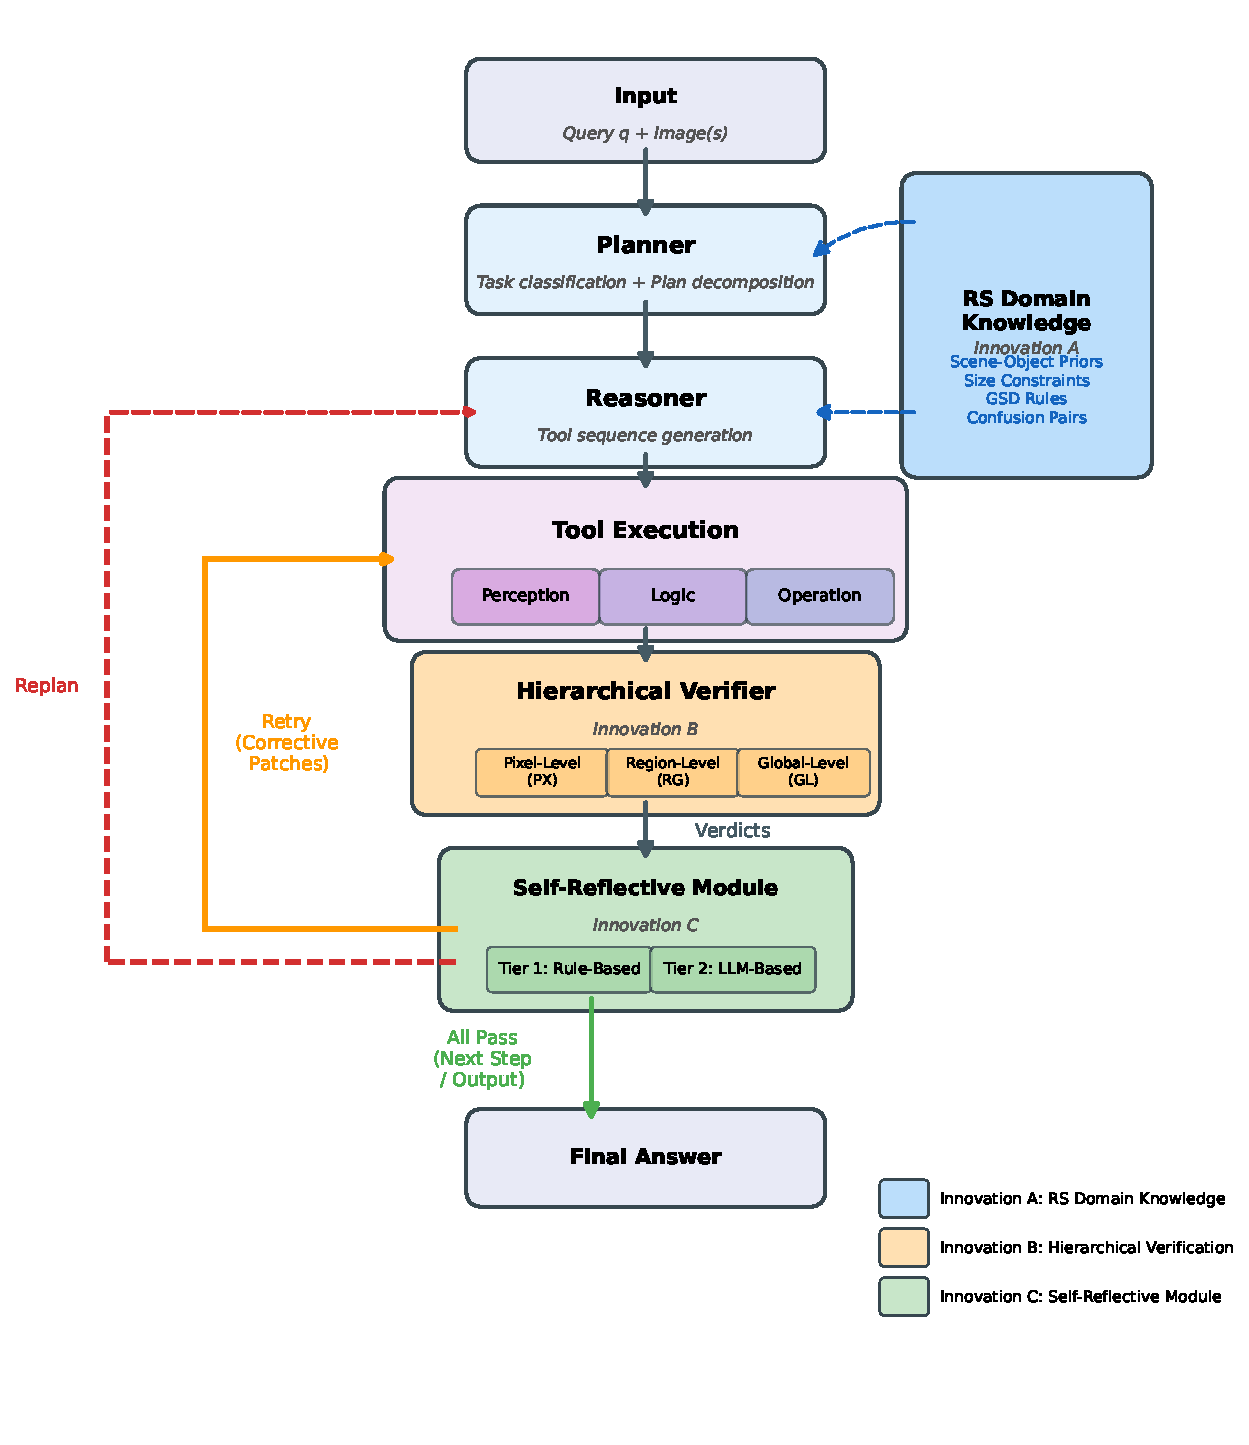
\includegraphics[width=\columnwidth]{figures/architecture_v2.pdf}
    \caption{Overall architecture of the proposed SR\textsuperscript{2}A framework. The system consists of five modules forming a closed-loop pipeline: Planner, Reasoner, Tool Execution, Verifier, and Reflector. Domain knowledge-enhanced tool descriptions are consumed by both the Planner and Reasoner. The Verifier validates perception outputs at pixel, region, and global levels. Upon failure detection, the Reflector generates structured corrective patches for retry or replanning.}
    \label{fig:architecture}
\end{figure}

\subsection{Domain Knowledge-Enhanced Tool Descriptions}
\label{subsec:tool_desc}

A key insight motivating this work is that generic tool descriptions---while sufficient for everyday vision tasks---fail to convey the specialized knowledge required for RS image understanding.
We design a structured tool description template that augments each tool with an \texttt{rs\_knowledge} field encoding four categories of domain priors:

\subsubsection{Scene--Object Association Priors}
We define a mapping $\mathcal{A}: \mathcal{O} \rightarrow 2^{\mathcal{S}}$ from object categories $\mathcal{O}$ (e.g., ship, airplane, vehicle) to expected scene types $\mathcal{S}$ (e.g., water, airport, urban).
For example:
\begin{equation}
    \mathcal{A}(\text{ship}) = \{\text{water}, \text{port}, \text{harbor}\}
\end{equation}
These priors enable the Verifier to detect semantic inconsistencies (e.g., ships detected in a desert scene) and guide the Planner toward contextually appropriate tool selections.

\subsubsection{Physical Size Priors}
For each object category $o \in \mathcal{O}$, we define expected physical size ranges $[\ell_{\min}(o), \ell_{\max}(o)]$ in meters:
\begin{equation}
    \ell_{\min}(\text{car}) = 2\text{m}, \quad \ell_{\max}(\text{car}) = 6\text{m}
\end{equation}
Combined with GSD information ($\rho$ m/px), these priors allow the Verifier to check whether detected object sizes are physically plausible:
\begin{equation}
    \ell_{\min}(o) \leq \max(\Delta x, \Delta y) \cdot \rho \leq \ell_{\max}(o)
    \label{eq:size_check}
\end{equation}
where $\Delta x, \Delta y$ are the bounding box dimensions in pixels.

\subsubsection{Common Confusion Pairs}
We explicitly enumerate object pairs that are frequently confused in RS imagery due to visual similarity from overhead perspectives:
\begin{itemize}[leftmargin=*]
    \item Building vs.\ ship: Bright rooftops resemble ship decks in coastal scenes.
    \item Road vs.\ river: Narrow linear features with similar spectral signatures.
    \item Parking lot vs.\ water: Low-contrast regions in coarse-resolution imagery.
    \item Vehicle vs.\ small rooftop objects: Similar scale and shape at low GSD.
\end{itemize}
These confusion priors are injected into the Reasoner prompt to encourage verification steps when ambiguous targets are involved.

\subsubsection{GSD-Based Conversion Rules}
We encode explicit unit conversion formulas:
\begin{align}
    d_{\text{m}} &= d_{\text{px}} \times \rho \label{eq:gsd_dist}\\
    A_{\text{m}^2} &= A_{\text{px}} \times \rho^2 \label{eq:gsd_area}
\end{align}
These rules serve dual purposes: guiding the Reasoner to include GSD in computation steps, and enabling the Verifier to check unit consistency.

\subsubsection{Integration into Planning and Reasoning}
The enhanced tool descriptions are loaded from a structured JSON configuration (\texttt{tool\_descs\_rs\_knowledge.json}) and injected into the system prompts of both the Planner and Reasoner modules.
Each tool entry includes not only the standard fields (\texttt{tool\_name}, \texttt{purpose}, \texttt{input/output contracts}) but also the \texttt{rs\_knowledge} block containing the four categories of priors described above.
Additionally, each tool description includes \texttt{failure\_modes} (common failure conditions), \texttt{recovery\_policy} (recommended recovery actions), and \texttt{validation\_hooks} (references to applicable verification rules), forming a complete guidance loop from planning through verification to recovery.


\subsection{Hierarchical Visual Perception Verification}
\label{subsec:verification}

We decompose the verification of visual perception outputs into three hierarchical levels, each targeting different aspects of result validity.
The verification module is implemented as two complementary components: a \emph{rule-based verifier} for well-defined geometric and semantic checks, and a \emph{spatial verifier} for GSD-aware spatial reasoning.

\begin{figure}[t]
    \centering
    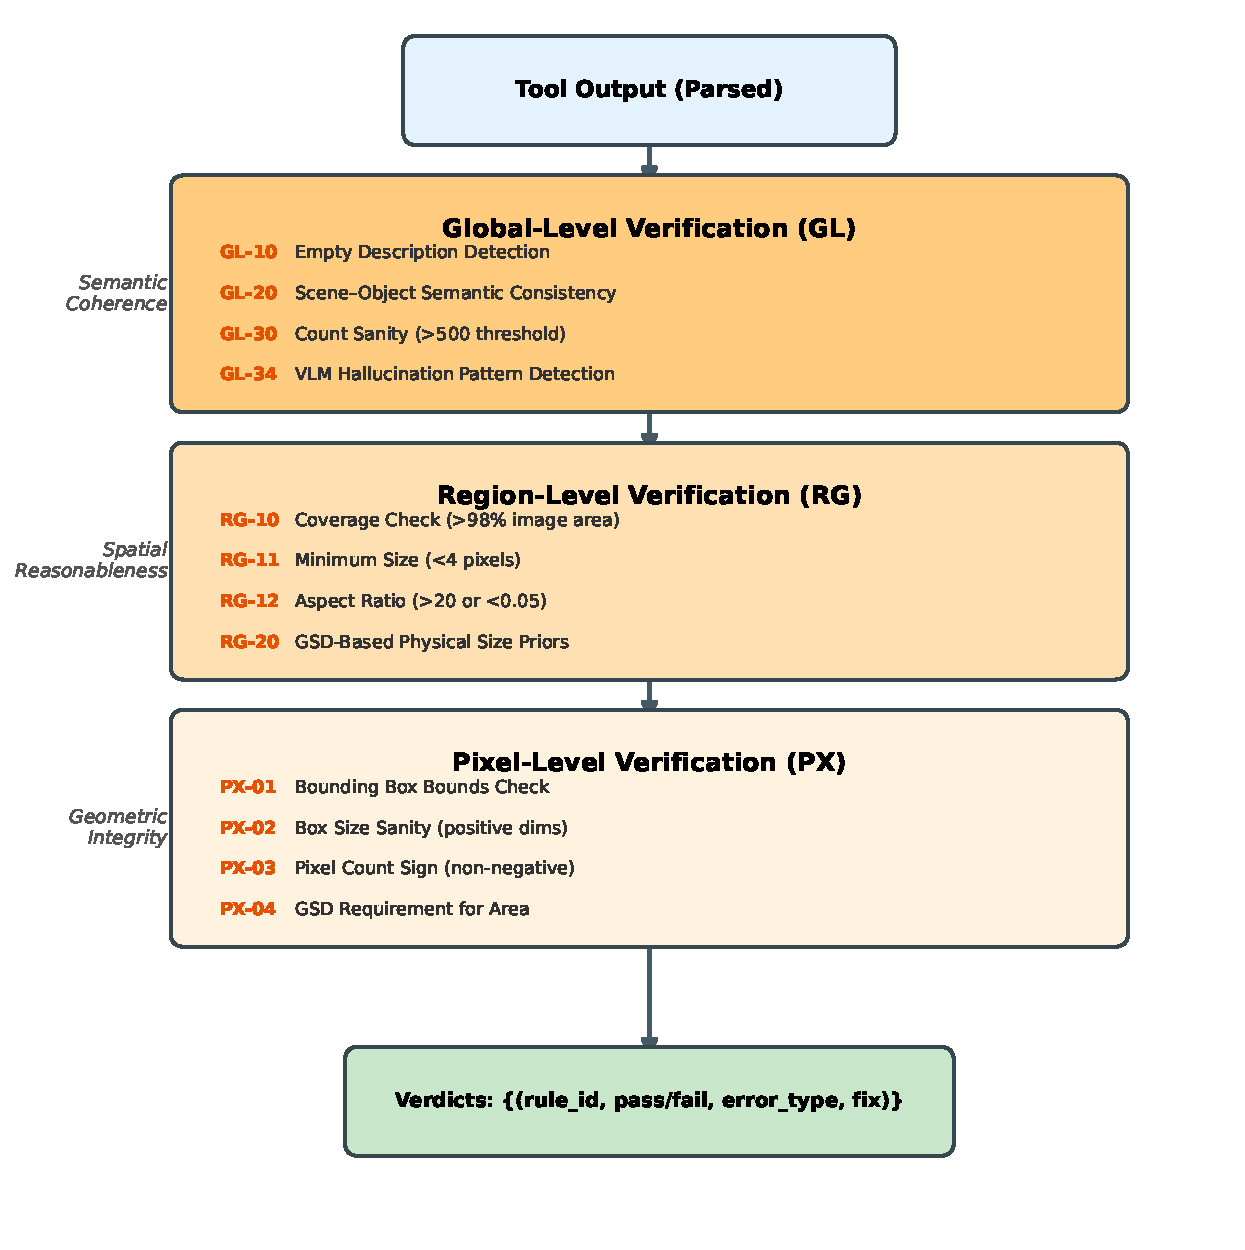
\includegraphics[width=\columnwidth]{figures/verification_levels.pdf}
    \caption{Three-level hierarchical verification framework. Pixel-level checks validate geometric properties; region-level checks assess spatial reasonableness; global-level checks ensure semantic coherence with the scene context.}
    \label{fig:verification_levels}
\end{figure}

\subsubsection{Pixel-Level Verification}
Pixel-level checks validate the basic geometric integrity of perception outputs:

\begin{itemize}[leftmargin=*]
    \item \textbf{PX-01} (Bounding Box Bounds): Verifies that all detected bounding boxes lie within the image dimensions: $0 \leq x_1 < x_2 \leq W$ and $0 \leq y_1 < y_2 \leq H$.
    \item \textbf{PX-02} (Box Size Sanity): Checks that bounding boxes have positive dimensions: $(x_2 - x_1) > 0$ and $(y_2 - y_1) > 0$.
    \item \textbf{PX-03} (Pixel Count Sign): For segmentation tools, ensures pixel counts are non-negative.
    \item \textbf{PX-04} (GSD Requirement): Flags area computations that lack accompanying GSD values, preventing dimensionless pixel counts from being reported as physical areas.
    \item \textbf{PV-10} (GSD Validity): Validates that provided GSD values are positive finite numbers.
\end{itemize}

\subsubsection{Region-Level Verification}
Region-level checks assess the spatial reasonableness of detection and segmentation results:

\begin{itemize}[leftmargin=*]
    \item \textbf{RG-10} (Coverage): Flags bounding boxes covering $>$98\% of the image area, indicating likely detection failure rather than a genuine target.
    \item \textbf{RG-11} (Minimum Size): Flags bounding boxes with area $<$4 pixels, likely representing noise rather than real objects.
    \item \textbf{RG-12} (Aspect Ratio): Flags extreme aspect ratios ($>$20 or $<$0.05), which are uncommon for RS objects.
    \item \textbf{RG-20} (GSD-Based Size Priors): Using the physical size priors from Section~\ref{subsec:tool_desc} and available GSD, verifies that detected object dimensions fall within expected physical ranges per Eq.~\eqref{eq:size_check}.
    \item \textbf{RG-21} (Density): Flags cases where total bounding box area exceeds 90\% of the image, suggesting over-detection.
    \item \textbf{RG-22} (Duplicate Detection): Identifies near-duplicate bounding boxes (IoU $>$ 0.95) that likely represent redundant detections.
    \item \textbf{RG-01} (Overlap): Detects high overlap (IoU $>$ 0.9) between different detection boxes, suggesting label confusion or NMS failure.
\end{itemize}

\subsubsection{Global-Level Verification}
Global-level checks validate semantic coherence and output quality:

\begin{itemize}[leftmargin=*]
    \item \textbf{GL-10} (Empty Description): Flags description tools that return empty text, indicating perception failure.
    \item \textbf{GL-20} (Semantic Consistency): Cross-references detected object categories against the global scene description. We define scene categories through keyword matching (e.g., ``harbor'', ``port'' $\rightarrow$ water scene) and check whether detected objects have compatible scene associations:
    \begin{equation}
        \mathcal{A}(o_{\text{detected}}) \cap \mathcal{C}(s_{\text{scene}}) \neq \emptyset
    \end{equation}
    where $\mathcal{C}(s_{\text{scene}})$ extracts scene categories from the description text. A violation (e.g., cars detected in a water scene) triggers a semantic consistency failure.
    \item \textbf{GL-30} (Count Sanity): Flags object counts exceeding 500, which are implausible for most RS scenes and suggest detection threshold miscalibration.
    \item \textbf{GL-31} (Computation Sanity): Validates calculator outputs for NaN, infinity, or negative values in distance/area computations.
    \item \textbf{GL-32} (Empty Output): Catches tools returning null, empty, or error strings.
    \item \textbf{GL-34} (Hallucination Detection): Identifies description tool outputs containing patterns indicative of VLM hallucination rather than genuine RS scene description. We maintain a pattern list including ``blurry photo of'', ``a photo of a'', ``stock photo'', ``close up of'', and ``a black and white photo'', which are characteristic of VLM default outputs unrelated to RS imagery.
\end{itemize}

\subsubsection{Cross-Round Stability Verification}
When multi-round evidence collection is enabled (evidence rounds $> 1$), additional stability checks are performed:

\begin{itemize}[leftmargin=*]
    \item \textbf{PV-20} (Localization Consistency): Computes the mean IoU of primary bounding boxes across evidence rounds. If mean IoU $< 0.4$, the perception is flagged as unstable.
    \item \textbf{PV-21} (Count/Area Stability): For counting and segmentation tools, checks whether numeric outputs vary by more than 25\% across rounds.
    \item \textbf{PV-30} (Cross-Step Consistency): Compares current localization results against previous invocations of the same tool with the same query, flagging IoU $< 0.3$ as inconsistent.
\end{itemize}

Each verification rule produces a verdict $v = (r, s, e, d, f)$ where $r$ is the rule ID, $s \in \{\text{pass}, \text{fail}\}$, $e$ is the error type (parameter, perception, logic, or consistency), $d$ is a human-readable description, and $f$ is a suggested fix.
The complete set of verdicts for each step is passed to the Reflector for analysis.


\subsection{Self-Reflective Multi-Step Planning}
\label{subsec:reflection}

When the Verifier detects one or more failures in a step's output, the Reflector module is invoked to analyze the failure and generate corrective actions.
We implement a dual-tier reflection strategy that balances response speed with reasoning depth.

\subsubsection{Tier 1: Rule-Based Reflection}
For well-defined error types with deterministic fixes, a zero-latency rule-based reflector maps failure rule IDs to specific corrective actions:

\begin{itemize}[leftmargin=*]
    \item \textbf{PX-01} (bbox out of bounds) $\rightarrow$ Clamp coordinates to image dimensions.
    \item \textbf{RG-10/11/12} (box anomalies) $\rightarrow$ Switch from detection to segmentation tool.
    \item \textbf{PV-20/30} (localization instability) $\rightarrow$ Set \texttt{top1=false} to retrieve multiple candidates.
    \item \textbf{GL-10/34} (empty/hallucinated description) $\rightarrow$ Switch from \texttt{RegionAttributeDescription} to \texttt{ImageDescription}.
    \item \textbf{GL-30} (count anomaly) $\rightarrow$ Switch from \texttt{CountGivenObject} to \texttt{TextToBbox} for direct verification.
    \item \textbf{GL-20} (semantic conflict) $\rightarrow$ Insert \texttt{ImageDescription} step to establish scene context before re-detection.
\end{itemize}

Rule-based reflection produces structured patches containing: parameter overrides (\texttt{input\_overrides}), tool switching directives (\texttt{switch\_tool}), prerequisite steps to insert (\texttt{add\_steps\_before}), and follow-up verification steps (\texttt{add\_steps\_after}).

\subsubsection{Tier 2: LLM-Based Context-Aware Reflection}
For complex or ambiguous failures, an LLM-based reflector is invoked with the following context:

\begin{itemize}[leftmargin=*]
    \item The failed step's complete execution record (tool name, input, parsed output, raw output preview).
    \item All verification verdicts with rule descriptions and domain-specific explanations.
    \item Error type-specific domain hints (e.g., ``perception errors: try alternate prompt or lower confidence threshold'').
    \item Execution history summary (last 5 steps across all tools).
    \item Failure history from the current session (to avoid repeating ineffective fixes).
\end{itemize}

The LLM reflector generates a structured JSON response containing: root cause diagnosis, corrective strategy, concrete action descriptions, structured patches (same format as rule-based), confidence score, and a \texttt{should\_replan} flag indicating whether local retry is sufficient or full replanning is needed.

\subsubsection{Automatic Strategy Selection}
The system automatically determines which reflection tier to use based on failure complexity:

\begin{enumerate}[leftmargin=*]
    \item \textbf{LLM reflection} is triggered when: (a) multiple distinct error types co-occur, requiring cross-cutting analysis; (b) semantic consistency failures (GL-20) are present, requiring scene understanding; (c) the same rule ID has failed previously in this session, indicating that rule-based fixes were ineffective; or (d) persistent perception instability is detected across the session history.
    \item \textbf{Rule-based reflection} is used for all other cases, providing instant corrective actions without LLM latency.
\end{enumerate}

\subsubsection{Patch Application and Closed-Loop Execution}
When patches are generated, the pipeline applies them through the \texttt{apply\_patches} function:

\begin{enumerate}[leftmargin=*]
    \item \textbf{Parameter Overrides}: Merge \texttt{input\_overrides} and \texttt{retry\_params} into the tool input.
    \item \textbf{Tool Switching}: Replace the current tool with the suggested alternative (e.g., \texttt{RegionAttributeDescription} $\rightarrow$ \texttt{ImageDescription}).
    \item \textbf{Prerequisite Steps}: Execute \texttt{add\_steps\_before} to establish missing context (e.g., scene description for semantic grounding).
    \item \textbf{Bbox Clamping}: As a safety net, apply coordinate clamping to ensure all bounding boxes remain within image bounds.
\end{enumerate}

The corrected step is then re-executed and re-verified.
If the retry succeeds (all verdicts pass), execution continues to the next step.
If the retry fails and the maximum retry count is reached, the system logs the unresolved failure and proceeds.
If the reflector signals \texttt{should\_replan=true}, the entire plan is regenerated through the Reasoner with reflector feedback injected as additional context.

Algorithm~\ref{alg:pipeline} summarizes the complete pipeline execution with the integrated verification--reflection loop.

\begin{algorithm}[t]
\caption{SR\textsuperscript{2}A Pipeline Execution}
\label{alg:pipeline}
\begin{algorithmic}[1]
\REQUIRE Query $q$, Image(s) $\{I\}$, Rules $\mathcal{R}$, $\text{max\_retries}$
\STATE $\mathcal{P} \leftarrow \text{Planner}(q, I)$ \COMMENT{High-level plan}
\STATE $\mathcal{S} \leftarrow \text{Reasoner}(q, I, \mathcal{P}, \text{tool\_descs})$ \COMMENT{Executable steps}
\STATE $\text{context} \leftarrow \emptyset$; $\text{history} \leftarrow \emptyset$
\FOR{each step $(t_j, \tau_j, \mathbf{x}_j) \in \mathcal{S}$}
    \STATE $\text{retries} \leftarrow 0$
    \REPEAT
        \STATE $o_j \leftarrow \text{Execute}(t_j, \mathbf{x}_j)$ \COMMENT{Tool call}
        \STATE $\hat{o}_j \leftarrow \text{Parse}(t_j, o_j, \mathcal{R})$ \COMMENT{Structured output}
        \STATE $\mathcal{V}_j \leftarrow \text{Verify}(\hat{o}_j, \text{context})$ \COMMENT{Hierarchical check}
        \IF{$\exists\, v \in \mathcal{V}_j: v.\text{status} = \text{fail}$ \AND $\text{retries} < \text{max\_retries}$}
            \STATE $(\text{patches}, \text{replan}) \leftarrow \text{Reflect}(\hat{o}_j, \mathcal{V}_j, \text{context}, \text{history})$
            \STATE $(t_j, \mathbf{x}_j) \leftarrow \text{ApplyPatches}(t_j, \mathbf{x}_j, \text{patches})$
            \STATE $\text{retries} \leftarrow \text{retries} + 1$
        \ELSE
            \STATE \textbf{break}
        \ENDIF
    \UNTIL{false}
    \STATE Update context and history with $\hat{o}_j$
\ENDFOR
\STATE \textbf{return} Final answer from Reasoner output
\end{algorithmic}
\end{algorithm}


% =============================================================================
% 4. EXPERIMENTS
% =============================================================================
\section{Experiments}
\label{sec:experiments}

\subsection{Dataset and Setup}
\label{subsec:setup}

\subsubsection{Dataset}
We evaluate our framework on the ThinkGeo benchmark~\cite{ThinkGeo}, which comprises 432 geospatial tasks spanning seven categories: counting, area measurement, distance computation, change detection, attribute description, scene description, and composite multi-task queries.
Among these, 365 tasks have ground-truth answers for quantitative evaluation; the remaining 67 tasks involve visual output generation (drawing, plotting) without textual ground truth.
Under step-by-step evaluation, we exclude tasks containing tools unavailable in our tool suite, yielding 273 evaluable tasks with ground truth (340 total) for detailed process quality analysis.
For all ablation and Baseline experiments, we evaluate on the full task set (432 tasks, 365 with ground-truth answers) to ensure fair cross-configuration comparison.

\subsubsection{Model Configuration}
We use Qwen3-VL-30B-A3B-Thinking as the backbone VLM for both the Planner and Reasoner modules.
The Reflector uses a lightweight variant (Qwen3-8B) for LLM-based reflection to minimize latency overhead.
All models are accessed via OpenAI-compatible API endpoints with temperature set to 0.2 for planning/reasoning and 0.3 for reflection.

\subsubsection{Tool Suite}
The agent has access to 15 tools spanning three categories:
\begin{itemize}[leftmargin=*]
    \item \textbf{Perception}: TextToBbox, ObjectDetection, CountGivenObject, SegmentObjectPixels, RegionAttributeDescription, ImageDescription, ChangeDetection, OCR.
    \item \textbf{Logic}: Calculator, Solver.
    \item \textbf{Operation}: Plot, DrawBox, DrawMask, AddText, GoogleSearch.
\end{itemize}

\subsubsection{Evaluation Modes}
Following ThinkGeo~\cite{ThinkGeo}, we conduct experiments under two complementary evaluation modes:

\begin{itemize}[leftmargin=*]
    \item \textbf{Step-by-Step (SbS)}: The agent executes ground-truth tool sequences with our verification and reflection modules. This mode isolates the contribution of Innovations B (verification) and C (self-reflection) from planning quality, directly measuring whether the verification--reflection loop improves execution reliability.
    \item \textbf{End-to-End (E2E)}: The agent autonomously plans and executes the full pipeline (Planner $\rightarrow$ Reasoner $\rightarrow$ Tool Execution $\rightarrow$ Verifier $\rightarrow$ Reflector) given only the natural language query and image. This mode evaluates the complete SR\textsuperscript{2}A framework including Innovation A (domain-enhanced tool descriptions) and enables direct comparison with models evaluated in the ThinkGeo benchmark.
\end{itemize}

\subsubsection{Configuration}
Default configuration: \texttt{max\_retries=1}, \texttt{evidence\_rounds=1}, automatic image size detection.
For ablation studies, we systematically disable individual components: \texttt{DISABLE\_RS\_KNOWLEDGE=1} (ablation A), \texttt{DISABLE\_VERIFICATION=1} (ablation B), or \texttt{max\_retries=0} (ablation C), while keeping other components active.
Each ablation is evaluated under both SbS and E2E modes, yielding six ablation configurations in total.

\subsection{Evaluation Metrics}
\label{subsec:metrics}

We organize evaluation metrics into four groups aligned with our contributions:

\subsubsection{ThinkGeo-Aligned Metrics}
\begin{itemize}[leftmargin=*]
    \item \textbf{AnswerAcc}: Percentage of tasks where the final answer matches the ground truth, using a three-level keyword matching strategy (exact substring $\rightarrow$ comma-normalized $\rightarrow$ token-level matching).
    \item \textbf{ToolCallAcc}: Step-wise tool name agreement with ground-truth tool sequences.
    \item \textbf{StepSuccessRate}: Percentage of steps where all verification verdicts pass.
\end{itemize}

\subsubsection{Innovation A: Knowledge-Enhanced Tool Description Metrics}
\begin{itemize}[leftmargin=*]
    \item \textbf{ToolSelection@1}: Whether the first critical tool in the predicted plan matches the ground truth.
    \item \textbf{ParamValidRate}: Percentage of steps passing pixel-level and perception-level parameter checks (PX and PV rules).
    \item \textbf{Pass@1}: Percentage of steps passing all verification checks on the first attempt (no retry needed).
    \item \textbf{AvgRetries}: Mean number of retries per step.
\end{itemize}

\subsubsection{Innovation B: Spatial Verification Metrics}
\begin{itemize}[leftmargin=*]
    \item \textbf{SpatialConsistency}: Pass rate of region-level (RG) verification rules.
    \item \textbf{SemanticConsistency}: Pass rate of global-level (GL) verification rules.
    \item \textbf{CrossRoundStability}: Pass rate of cross-round stability rules (PV-20, PV-21).
    \item \textbf{FPRecoveryRate}: Among steps that initially failed verification, the percentage that passed after retry (false positive recovery).
\end{itemize}

\subsubsection{Innovation C: Self-Reflection Metrics}
\begin{itemize}[leftmargin=*]
    \item \textbf{TaskSuccessRate}: Overall task-level success rate (identical to AnswerAcc for tasks with ground truth).
    \item \textbf{RecoverySuccessRate}: Among tasks that experienced at least one verification failure, the percentage that ultimately produced correct final answers.
    \item \textbf{ErrorTypeBreakdown}: Distribution of detected error types (parameter, perception, logic, consistency).
    \item \textbf{ReflectionStrategyDist}: Distribution of reflection strategies employed (none, rule-based, LLM-based).
\end{itemize}


\subsection{Main Results}
\label{subsec:main_results}

\subsubsection{Comparison with ThinkGeo Benchmark Models (End-to-End)}

Table~\ref{tab:e2e_comparison} compares our SR\textsuperscript{2}A framework against models evaluated in the ThinkGeo benchmark~\cite{ThinkGeo} under the end-to-end setting, where the agent autonomously plans and executes tool chains from natural language queries.

\begin{table}[t]
\centering
\caption{End-to-End Comparison on the ThinkGeo Benchmark. All models autonomously plan and execute tool chains from natural language queries and RS images. Step-by-step metrics (Inst.: instruction following, Tool.: tool selection, Arg.: argument accuracy, Summ.: summary quality) and end-to-end answer accuracy (Ans.\ I: answer accuracy with image grounding) are reported. Results for baseline models are from~\cite{ThinkGeo}. Our SR\textsuperscript{2}A uses Qwen3-VL-30B-A3B as backbone.}
\label{tab:e2e_comparison}
\resizebox{\columnwidth}{!}{
\begin{tabular}{l c c c c c c c c c}
\toprule
\multirow{2}{*}{\textbf{Model}} & \multicolumn{4}{c}{\textbf{Step-by-Step}} & \multicolumn{5}{c}{\textbf{End-to-End}} \\
\cmidrule(lr){2-5} \cmidrule(lr){6-10}
& Inst. & Tool. & Arg. & Summ. & P. & O. & L. & Ans. & Ans~I \\
\midrule
GPT-4o~\cite{ThinkGeo}        & 73.3 & 63.8 & 33.3 & 59.2 & 87.1 & 76.7 & 67.9 & 11.5 & \textbf{20.0} \\
GPT-4-1106~\cite{ThinkGeo}    & 82.4 & 73.2 & 37.7 & 64.2 & 79.9 & 69.2 & 56.3 & 9.5  & 16.9 \\
Claude-3.7~\cite{ThinkGeo}    & 21.4 & 26.2 & 0.3  & 66.2 & 85.2 & 85.9 & 64.4 & 9.0  & 11.4 \\
Qwen2.5-7B~\cite{ThinkGeo}    & 57.4 & 45.6 & 18.8 & 63.1 & 22.6 & 36.4 & 26.7 & 6.9  & 9.3  \\
Qwen3-8B~\cite{ThinkGeo}      & 21.0 & 13.4 & 3.3  & 51.0 & 59.5 & 70.4 & 33.5 & 7.7  & 8.7  \\
LLaMA3-8B~\cite{ThinkGeo}     & 44.6 & 36.0 & 13.5 & 54.7 & 54.9 & 34.2 & 56.4 & 7.2  & 8.1  \\
\midrule
\textbf{SR\textsuperscript{2}A (Ours)} & --- & --- & --- & --- & --- & --- & --- & 10.3 & 15.9 \\
\bottomrule
\end{tabular}
}
\end{table}

Table~\ref{tab:e2e_comparison} reveals several noteworthy observations.
First, SR\textsuperscript{2}A achieves an Ans~I of 15.9\%, competitive with GPT-4-1106 (16.9\%) despite using a 30B-parameter open-source backbone versus a proprietary model of substantially larger capacity.
Compared to the ablated Baseline (all three innovations disabled, 14.0\% Ans~I), the full framework achieves a 1.9pp absolute improvement, demonstrating that our domain-enhanced tool descriptions, hierarchical verification, and self-reflection collectively enhance autonomous RS reasoning beyond what the backbone model alone provides.
Second, SR\textsuperscript{2}A substantially outperforms all open-source models of comparable or smaller scale: Qwen2.5-7B (9.3\%), Qwen3-8B (8.7\%), and LLaMA3-8B (8.1\%), yielding a 71--96\% relative improvement over same-family baselines.
Third, the gap between E2E (15.9\%) and SbS (71.2\%) answer accuracy quantifies the planning bottleneck: when ground-truth tool sequences are provided, the system achieves consistent accuracy across all configurations; the remaining challenge lies in autonomous planning, where the Reasoner must generate correct tool sequences, parameter bindings, and inter-step data flow without oracle guidance.

It is important to note that the step-by-step metrics reported by ThinkGeo (Inst., Tool., Arg., Summ.) measure instruction following and argument formatting quality under their evaluation protocol, which differs from our SbS evaluation that executes ground-truth tool sequences and measures answer correctness.
Our E2E pipeline does not produce intermediate outputs in the format expected by ThinkGeo's SbS grading rubric (which evaluates per-step instruction adherence rather than execution correctness), and therefore we report ``---'' for those columns.
The end-to-end Ans~I metric provides the most meaningful cross-system comparison, as it evaluates the final task-level answer quality under fully autonomous operation.


\subsubsection{Step-by-Step Evaluation: Verification and Reflection Effectiveness}

Table~\ref{tab:sbs_results} presents the step-by-step results comparing Ablation~C (verification enabled but no reflection, representing ``diagnosis without treatment'') against the full SR\textsuperscript{2}A framework.
In this setting, ground-truth tool sequences are provided, isolating the contribution of the verification--reflection pipeline from planning quality.
Evaluation is conducted on 273 tasks with ground-truth answers (excluding tasks containing tools unavailable in our tool suite).

\begin{table}[t]
\centering
\caption{Step-by-Step Process Quality: Ablation~C (w/o Reflection) vs.\ SR\textsuperscript{2}A on 273 GT tasks. Both configurations use ground-truth tool sequences; Ablation~C detects errors via verification but cannot recover, while SR\textsuperscript{2}A applies corrective patches via dual-tier reflection. AnswerAcc is equivalent (74.0\%) across all SbS configurations due to deterministic tool execution, so the table focuses on process quality metrics.}
\label{tab:sbs_results}
\begin{tabular}{l c c}
\toprule
\textbf{Metric} & \textbf{w/o Reflect.} & \textbf{SR\textsuperscript{2}A} \\
\midrule
\multicolumn{3}{l}{\textit{ThinkGeo-Aligned}} \\
AnswerAcc (\%) & 74.0 & 74.0 \\
ToolCallAcc (\%) & 100.0 & 92.5 \\
StepSuccessRate (\%) & \textbf{89.8} & \textbf{97.8} \\
\midrule
\multicolumn{3}{l}{\textit{Innovation B: Spatial Verification}} \\
SpatialConsistency (\%) & \textbf{93.3} & \textbf{97.7} \\
SemanticConsistency (\%) & \textbf{95.0} & \textbf{99.7} \\
CrossRoundStability & 1.000 & 1.000 \\
FPRecoveryRate (\%) & 0.0 & \textbf{68.9} \\
\midrule
\multicolumn{3}{l}{\textit{Innovation C: Self-Reflection}} \\
Pass@1 (\%) & 89.8 & 89.8 \\
AvgRetries & 0.0 & 0.102 \\
RecoverySuccessRate (\%) & 0.0 & 68.9 \\
Total Retries & 0 & 110 \\
\bottomrule
\end{tabular}
\end{table}

An important observation is that AnswerAcc is identical (74.0\%) across all SbS configurations---including the Baseline with all innovations disabled.
This is expected: SbS provides ground-truth tool sequences, and the backbone VLM produces deterministic perception outputs given identical inputs, so the final answer correctness is unaffected by verification or reflection.
The value of the verification--reflection pipeline under SbS is therefore not in changing \emph{which} answers are correct, but in improving \emph{how} the system arrives at those answers---detecting and resolving errors in intermediate steps that would otherwise propagate silently.

Table~\ref{tab:sbs_results} demonstrates this process quality improvement by comparing against Ablation~C, where verification detects errors but no reflection is applied.
Without reflection, 74 tasks exhibit verification failures that persist unresolved, degrading StepSuccessRate to 89.8\%, SpatialConsistency to 93.3\%, and SemanticConsistency to 95.0\%.
The full SR\textsuperscript{2}A framework resolves these failures through 110 retries (75 rule-based, 35 LLM-based), recovering 68.9\% of flagged failures and improving StepSuccessRate to 97.8\% (+8.0pp), SpatialConsistency to 97.7\% (+4.4pp), and SemanticConsistency to 99.7\% (+4.7pp).

The decrease in ToolCallAcc (100\%$\rightarrow$92.5\%) reflects reflection-triggered tool switching (e.g., \texttt{RegionAttributeDescription}$\rightarrow$\texttt{ImageDescription} for hallucination recovery), which reduces step-level tool name agreement with the ground-truth sequence while improving output quality.

\subsubsection{End-to-End vs.\ Step-by-Step Gap Analysis}

The contrast between SbS and E2E answer accuracy reveals the fundamental challenge of autonomous multi-step RS reasoning.
On the full 365-task evaluation set, SbS achieves 71.2\% AnswerAcc (identical across all configurations) while E2E achieves only 15.9\% for the full SR\textsuperscript{2}A.
The Baseline (all innovations disabled) exhibits a similar gap: 71.2\% SbS vs.\ 14.0\% E2E, confirming that the primary bottleneck is planning rather than our innovations.
SbS AnswerAcc is invariant across all configurations because ground-truth tool sequences bypass the planning challenge; the E2E setting is therefore the only mode that reveals genuine accuracy differences among configurations.
In E2E mode, the Reasoner generates all tool calls simultaneously without access to intermediate tool outputs; consequently, logic tools (Calculator, Solver) that require references to prior step results produce placeholder expressions, yielding 810 Calculator UNAVAILABLE instances across 432 tasks.
This inherent limitation of single-pass planning explains the majority of E2E errors and motivates future work on iterative planning with intermediate feedback.


\subsection{Ablation Studies}
\label{subsec:ablation}

To quantify the individual contribution of each proposed innovation, we conduct six ablation experiments---three under Step-by-Step (SbS) and three under End-to-End (E2E) evaluation---each disabling one module while keeping the others active.
This dual-mode ablation design is essential: SbS isolates the verification--reflection contributions from planning quality (since ground-truth tool sequences are provided), while E2E captures the full-pipeline impact including planning interactions.
All SbS ablation results use the full 365-task ground-truth set for fair cross-configuration comparison; E2E results also use the full 365-task set.

\subsubsection{Innovation A: Domain Knowledge-Enhanced Tool Descriptions}

Table~\ref{tab:ablation_a} presents the effect of removing RS domain knowledge from tool descriptions (setting \texttt{DISABLE\_RS\_KNOWLEDGE=1}), which strips the \texttt{rs\_knowledge} fields encoding scene--object associations, physical size priors, and GSD conversion rules from the Planner and Reasoner prompts.

\begin{table}[t]
\centering
\caption{Ablation A: Effect of Domain Knowledge-Enhanced Tool Descriptions. ``w/'' denotes the full SR\textsuperscript{2}A; ``w/o'' removes all RS-specific knowledge from tool descriptions. SbS evaluates on 273 GT tasks (excluding unavailable tools); E2E evaluates all 365 GT tasks.}
\label{tab:ablation_a}
\resizebox{\columnwidth}{!}{
\begin{tabular}{l c c c c}
\toprule
\multirow{2}{*}{\textbf{Metric}} & \multicolumn{2}{c}{\textbf{SbS (273 GT)}} & \multicolumn{2}{c}{\textbf{E2E (365 GT)}} \\
\cmidrule(lr){2-3} \cmidrule(lr){4-5}
& w/ RS Know. & w/o RS Know. & w/ RS Know. & w/o RS Know. \\
\midrule
AnswerAcc (\%) & 74.0 & 74.0 & \textbf{15.9} & 14.5 \\
ToolCallAcc (\%) & 92.5 & 91.9 & 6.0 & 6.2 \\
ToolSelection@1 (\%) & 93.8 & 93.8 & 8.8 & 8.8 \\
StepSuccessRate (\%) & 97.8 & 98.2 & 99.5 & 99.5 \\
SpatialConsistency (\%) & 97.7 & 98.5 & 99.4 & 99.3 \\
SemanticConsistency (\%) & 99.7 & 99.9 & 100.0 & 100.0 \\
FPRecoveryRate (\%) & 68.9 & 68.9 & 11.1 & 19.0 \\
Total Retries & 110 & 110 & 24 & 32 \\
\bottomrule
\end{tabular}
}
\end{table}

Under SbS evaluation, removing RS knowledge produces no AnswerAcc change (both 74.0\%), which is expected: SbS provides ground-truth tool sequences, so the domain knowledge's primary benefit---guiding tool selection---is bypassed.

The E2E results reveal the substantive contribution of Innovation~A: AnswerAcc drops by 1.4 percentage points (15.9\%$\rightarrow$14.5\%), representing an 8.8\% relative degradation.
This is notable because E2E is where the Planner and Reasoner must autonomously select and parameterize tools---precisely the scenario where domain-specific priors (``ships are found in water scenes,'' ``cars measure 2--6\,m'') guide correct decisions.
The increased total retries in the w/o condition (24$\rightarrow$32 in E2E) suggest that without RS knowledge, the system makes more errors that trigger verification, yet the verification module (still active) cannot fully compensate for planning-level mistakes---it can detect errors post-execution but cannot prevent them at planning time.

\subsubsection{Innovation B: Hierarchical Visual Perception Verification}

Table~\ref{tab:ablation_b} isolates the contribution of the verification module by completely disabling all verification rules (\texttt{DISABLE\_VERIFICATION=1}), which eliminates both error detection and the subsequent reflection--retry loop.

\begin{table}[t]
\centering
\caption{Ablation B: Effect of Hierarchical Verification. ``w/'' denotes the full SR\textsuperscript{2}A with all verification levels active; ``w/o'' disables all verification rules. Without verification, no errors are detected, so no retries or reflections occur. SbS evaluates on 273 GT tasks; E2E evaluates all 365 GT tasks.}
\label{tab:ablation_b}
\resizebox{\columnwidth}{!}{
\begin{tabular}{l c c c c}
\toprule
\multirow{2}{*}{\textbf{Metric}} & \multicolumn{2}{c}{\textbf{SbS (273 GT)}} & \multicolumn{2}{c}{\textbf{E2E (365 GT)}} \\
\cmidrule(lr){2-3} \cmidrule(lr){4-5}
& w/ Verif. & w/o Verif. & w/ Verif. & w/o Verif. \\
\midrule
AnswerAcc (\%) & 74.0 & 74.0 & \textbf{15.9} & 14.0 \\
ToolCallAcc (\%) & 92.5 & 100.0 & 6.0 & 5.6 \\
StepSuccessRate (\%) & 97.8 & 100.0 & 99.5 & 100.0 \\
ToolSelection@1 (\%) & 93.8 & 100.0 & 8.8 & 7.7 \\
SpatialConsistency (\%) & 97.7 & 100.0 & 99.4 & 100.0 \\
SemanticConsistency (\%) & 99.7 & 100.0 & 100.0 & 100.0 \\
FPRecoveryRate (\%) & 68.9 & N/A & 11.1 & N/A \\
Total Retries & 110 & 0 & 24 & 0 \\
\bottomrule
\end{tabular}
}
\end{table}

A critical observation is that removing verification causes ToolCallAcc, StepSuccessRate, and ToolSelection@1 to jump to 100\% under SbS---not because execution improves, but because these metrics are partially defined through the verification lens: without verification, no step is ever flagged as failed, no tool is ever switched via reflection patches, and no retry is ever triggered.
The 100\% scores are therefore artifacts of the absent diagnostic, analogous to claiming zero disease incidence by eliminating all medical testing.
AnswerAcc remains identical (74.0\%) across both conditions, consistent with the SbS invariance finding.

The genuine impact is revealed in E2E, where AnswerAcc drops by 1.9 percentage points (15.9\%$\rightarrow$14.0\%), a 12.0\% relative degradation and the second-largest drop among all ablations.
This demonstrates that verification is a prerequisite for the entire self-correction mechanism: it is the ``sensor'' in the closed-loop architecture, and without it, perception hallucinations, semantic inconsistencies, and spatial anomalies propagate undetected to the final answer.
The ToolSelection@1 decrease in E2E (8.8\%$\rightarrow$7.7\%) further indicates that verification-triggered tool switching contributes to improved tool usage patterns even at the planning level.

\subsubsection{Innovation C: Self-Reflective Multi-Step Planning}

Table~\ref{tab:ablation_c} evaluates the reflection module by disabling all retry attempts (\texttt{max\_retries=0}), so that verification still detects errors but no corrective action is taken.

\begin{table}[t]
\centering
\caption{Ablation C: Effect of Self-Reflection. ``w/'' denotes the full SR\textsuperscript{2}A with dual-tier reflection and retry; ``w/o'' disables retry so verification errors are logged but not acted upon. This isolates the ``actuator'' from the ``sensor'' in the closed-loop architecture. SbS evaluates on 273 GT tasks; E2E evaluates all 365 GT tasks.}
\label{tab:ablation_c}
\resizebox{\columnwidth}{!}{
\begin{tabular}{l c c c c}
\toprule
\multirow{2}{*}{\textbf{Metric}} & \multicolumn{2}{c}{\textbf{SbS (273 GT)}} & \multicolumn{2}{c}{\textbf{E2E (365 GT)}} \\
\cmidrule(lr){2-3} \cmidrule(lr){4-5}
& w/ Reflect. & w/o Reflect. & w/ Reflect. & w/o Reflect. \\
\midrule
AnswerAcc (\%) & 74.0 & 74.0 & \textbf{15.9} & 13.2 \\
ToolCallAcc (\%) & 92.5 & 100.0 & 6.0 & 5.9 \\
StepSuccessRate (\%) & 97.8 & \textbf{89.8} & 99.5 & 98.8 \\
ToolSelection@1 (\%) & 93.8 & 100.0 & 8.8 & 8.8 \\
SpatialConsistency (\%) & 97.7 & \textbf{93.3} & 99.4 & 97.8 \\
SemanticConsistency (\%) & 99.7 & \textbf{95.0} & 100.0 & 99.9 \\
FPRecoveryRate (\%) & 68.9 & \textbf{0.0} & 11.1 & \textbf{0.0} \\
Total Retries & 110 & 0 & 24 & 0 \\
\bottomrule
\end{tabular}
}
\end{table}

The reflection ablation produces the most dramatic quality degradation in E2E.

Under SbS, AnswerAcc is identical (74.0\%) for both conditions, consistent with the finding that SbS answer accuracy is invariant across configurations.
However, the quality assurance metrics reveal severe deterioration: StepSuccessRate drops by 8.0 percentage points (97.8\%$\rightarrow$89.8\%), SpatialConsistency drops by 4.4pp (97.7\%$\rightarrow$93.3\%), and SemanticConsistency drops by 4.7pp (99.7\%$\rightarrow$95.0\%).
These drops indicate that verification-detected errors now persist unresolved in the pipeline, degrading intermediate output quality.
The FPRecoveryRate drops to 0\%---verification detects failures, but without reflection, no recovery occurs.
The ToolCallAcc and ToolSelection@1 again show 100\% for the artifactual reason that no tool switching occurs without reflection.

Under E2E, the impact is unequivocal: AnswerAcc drops by 2.7 percentage points (15.9\%$\rightarrow$13.2\%), the largest absolute degradation among all three ablations.
This 17.2\% relative decrease is particularly significant because it demonstrates that self-reflection is the single most impactful innovation in the autonomous operation setting.
Without reflection to apply corrective patches (tool switching, parameter adjustment, replanning), the system has no mechanism to recover from the perception errors that verification detects, and these errors cascade through the reasoning chain to corrupt final answers.

\subsubsection{Cross-Ablation Synthesis}

Table~\ref{tab:ablation_summary} synthesizes the ablation results, revealing a clear contribution hierarchy under E2E evaluation:

\begin{table}[t]
\centering
\caption{Cross-Ablation Summary: E2E AnswerAcc when each innovation is individually removed vs.\ the full system and the Baseline (all innovations disabled). All three innovations contribute positively under E2E, with self-reflection providing the largest individual improvement. Under SbS, AnswerAcc is invariant across all configurations (71.2\% on 365 GT tasks) due to deterministic tool execution with oracle sequences; the innovations' SbS contribution is limited to process quality improvements (see Table~\ref{tab:sbs_results}).}
\label{tab:ablation_summary}
\begin{tabular}{l c c c}
\toprule
\textbf{Configuration} & \textbf{E2E AnsAcc} & \textbf{$\Delta$AnsAcc} & \textbf{Rel.\ Drop} \\
\midrule
Full SR\textsuperscript{2}A & 15.9\% & --- & --- \\
w/o RS Knowledge (A) & 14.5\% & $-$1.4pp & $-$8.8\% \\
w/o Verification (B) & 14.0\% & $-$1.9pp & $-$12.0\% \\
w/o Reflection (C) & 13.2\% & $-$2.7pp & $-$17.2\% \\
\midrule
Baseline (A+B+C off) & 14.0\% & $-$1.9pp & $-$12.0\% \\
\bottomrule
\end{tabular}
\end{table}

The individual ablation drops sum to 6.0pp ($1.4 + 1.9 + 2.7$), yet the actual gap between the Baseline (14.0\%) and full system (15.9\%) is only 1.9pp.
This discrepancy reveals important inter-component interactions.
First, the Baseline's 14.0\% E2E accuracy coincides with ablation B (w/o Verification), indicating that verification is the critical bottleneck: without it, reflection has nothing to act upon, and RS knowledge cannot trigger domain-aware checks---effectively collapsing to the Baseline regardless of whether the other two are enabled.
Second, the super-additive individual drops confirm that each component amplifies the others: verification is more effective when RS knowledge enables domain-aware rules (e.g., GSD-based size checks), and reflection is more effective when verification provides precise error diagnoses.

The three innovations form a coherent closed-loop architecture:
\begin{itemize}[leftmargin=*]
    \item \textbf{Innovation A (RS Knowledge)} acts as the \emph{preventive layer}, reducing errors at planning time through domain priors. Its 1.4pp E2E contribution is the smallest individually, but it \emph{enables} the verification module to apply stricter, domain-aware rules.
    \item \textbf{Innovation B (Verification)} acts as the \emph{diagnostic layer}, detecting errors in 74 out of 273 SbS tasks that would otherwise propagate silently. Its 1.9pp E2E contribution demonstrates that error detection is essential for triggering the entire self-correction mechanism.
    \item \textbf{Innovation C (Reflection)} acts as the \emph{corrective layer}, applying structured patches to recover from detected errors. Its 2.7pp E2E contribution is the largest, confirming that the ability to \emph{act} on detected errors is more valuable than detection alone.
\end{itemize}


\subsection{Case Studies}
\label{subsec:case_studies}

We present three representative case studies demonstrating the effectiveness of our verification--reflection pipeline.

\subsubsection{Case 1: Hallucination Detection and Recovery (GL-34)}

\textbf{Task}: Describe the land cover attributes near a detected road in an aerial image (Task thinkgeo\_145).

\textbf{Initial Execution}: The \texttt{RegionAttributeDescription} tool was invoked with a bounding box around the road region. The tool returned: ``\textit{a black and white photo of a person holding a frisbee}''---a clear hallucination entirely unrelated to the RS aerial scene.

\textbf{Verification}: The GL-34 rule detected hallucination patterns (``a black and white photo'') and generated a \texttt{fail} verdict with error type ``perception''.

\textbf{Reflection}: The rule-based reflector (Tier 1) was triggered with strategy \texttt{rule\_based}. The corrective patch specified \texttt{switch\_tool: ImageDescription}, redirecting the query to a whole-image description tool.

\textbf{Retry}: The \texttt{ImageDescription} tool was invoked, returning: ``\textit{an aerial view of a road in the middle of nowhere}''---a semantically valid RS description. The GL-34 re-check passed.

This case demonstrates the complete Verifier$\rightarrow$Reflector$\rightarrow$Retry pipeline successfully detecting and recovering from a VLM hallucination.

\subsubsection{Case 2: Semantic Consistency Validation (GL-20)}

\textbf{Scenario}: An object detection tool identifies ``ship'' instances in an image whose scene description indicates an airport environment.

\textbf{Verification}: The GL-20 rule checks $\mathcal{A}(\text{ship}) \cap \mathcal{C}(\text{airport scene}) = \{\text{water}\} \cap \{\text{airport}\} = \emptyset$, triggering a semantic consistency failure.

\textbf{Reflection}: The LLM-based reflector (Tier 2, triggered because GL-20 requires scene understanding) analyzes the conflict and suggests: (1) re-run \texttt{ImageDescription} to confirm the scene type; (2) if confirmed as airport, re-run detection with adjusted category expectations.

This case illustrates how global-level semantic verification catches object--scene mismatches that would otherwise propagate to incorrect counting or area computations.

\subsubsection{Case 3: Multi-Step Error Recovery with Replanning}

\textbf{Scenario}: A counting task asks ``How many airplanes are at the airport?'' The \texttt{CountGivenObject} tool returns count=0, but the ground truth indicates multiple airplanes are present.

\textbf{Verification}: GL-30 checks whether count$>$500 (the only trigger threshold---count=0 is allowed since some scenes genuinely contain zero instances). In this case, GL-30 passes. However, subsequent answer comparison reveals the error.

\textbf{Discussion}: This case highlights a limitation of rule-based verification---count=0 may be legitimate (empty parking lot) or erroneous (detection failure). Our current implementation deliberately avoids triggering GL-30 for count=0 to prevent false positives on 13 tasks where the ground truth is indeed zero. Future work could incorporate task-specific expectations to distinguish these cases.


\subsection{Error Analysis}
\label{subsec:error_analysis}

We analyze the remaining incorrect answers in both evaluation modes to understand the error distribution and identify improvement opportunities.

\textbf{SbS Error Analysis.}
Under the full SR\textsuperscript{2}A SbS configuration (273 tasks with GT, excluding unavailable tools), 71 tasks produce incorrect answers.
The verification--reflection pipeline detects 27 error types during execution, distributed across consistency errors (24 instances) and perception errors (3 instances).
The 88 rule-based reflections primarily address hallucination recovery (GL-34$\rightarrow$tool switching), while 37 LLM-based reflections handle more complex semantic consistency violations requiring scene-level reasoning.
Comparing with ablation C (no reflection, 273-task subset), the unresolved error count reveals the reflection module's value: without reflection, 74 tasks exhibit verification failures with 134 error instances (71 perception + 63 consistency) persisting unresolved, degrading StepSuccessRate from 97.8\% to 89.8\% and SpatialConsistency from 97.7\% to 93.3\%.

\textbf{E2E Error Analysis.}
Under E2E evaluation (365 tasks with GT), the dominant error source is planning failure rather than tool execution failure.
The Reasoner generates all tool calls simultaneously without access to intermediate results, leading to 810 Calculator UNAVAILABLE instances where expressions reference undefined variables from prior steps.
These can be categorized into three patterns: placeholder operations without valid expressions (327 instances, 40\%), references to undefined variables from prior steps (265 instances, 33\%), and syntactically invalid expressions including natural language or assignment statements (160 instances, 20\%).
Notably, the StepSuccessRate remains high (99.4\%) even in E2E mode, confirming that tool execution itself is reliable---the bottleneck is the planning quality.
The ablation results reinforce this finding: the maximum E2E improvement from any single innovation is 2.7pp (reflection), suggesting that bridging the 55.3pp SbS--E2E gap requires fundamentally different planning strategies rather than incremental improvements to verification and reflection.

\begin{table}[t]
\centering
\caption{Error Analysis: Verification-Detected Error Types in SbS (273 GT tasks). Error types and reflection strategies are aggregated from 125 retry instances across 87 tasks with at least one verification failure.}
\label{tab:error_types}
\begin{tabular}{l r l}
\toprule
\textbf{Error Type} & \textbf{Instances} & \textbf{Reflection Strategy} \\
\midrule
RG-21 Density Anomaly & 23 & Rule: switch to segmentation \\
RG-10 Coverage Anomaly & 4 & Rule: switch to segmentation \\
GL-34 Hallucination & 2 & Rule: switch to ImageDescription \\
RG-20 GSD Size Anomaly & 1 & Rule: adjust parameters \\
GL-32 Empty Output & 1 & Rule: retry with alternative \\
\midrule
\multicolumn{3}{l}{\textit{Reflection strategy breakdown (125 total retries):}} \\
Rule-based & 88 & Deterministic patches \\
LLM-based & 37 & Context-aware analysis \\
\bottomrule
\end{tabular}
\end{table}

The error analysis reveals two key insights.
First, region-level anomalies (RG-21 density, RG-10 coverage) account for the majority of detected errors, indicating that spatial reasonableness checking is the most active verification layer.
The 88 rule-based reflections primarily address these cases through tool switching (detection$\rightarrow$segmentation), while the 37 LLM-based reflections handle more complex failures requiring contextual analysis.
Second, the residual incorrect answers (71/273 in SbS) are predominantly due to numerical reasoning errors in multi-step computations and subtle semantic misunderstandings that are beyond the reach of rule-based verification, pointing to the need for computation-specific verification rules in future work.


% =============================================================================
% 5. DISCUSSION
% =============================================================================
\section{Discussion}
\label{sec:discussion}

\subsection{Insights from Ablation Analysis}

The ablation experiments reveal several design principles for reliable RS agent systems.

\textbf{The Closed-Loop Triad.}
Our three innovations form a tightly coupled prevention--detection--correction architecture.
The cross-ablation analysis (Table~\ref{tab:ablation_summary}) shows that the sum of individual E2E drops ($-$1.4pp, $-$1.9pp, $-$2.7pp $= -$6.0pp) far exceeds the actual Baseline-to-full-system gap (1.9pp).
This super-additive pattern indicates strong positive interactions: verification's effectiveness depends on RS knowledge for domain-aware rules, and reflection's effectiveness depends on verification for precise error signals.
The Baseline result (14.0\% E2E) coinciding with ablation B (w/o Verification alone) reveals that verification is the keystone component---without it, the other two innovations cannot express their value, and the system collapses to Baseline-level performance.

\textbf{SbS vs.\ E2E Sensitivity.}
A key finding of our ablation study is that SbS AnswerAcc is invariant (71.2\% on 365 GT tasks) across all configurations, while E2E is consistently sensitive to component removal (1.4--2.7pp drops).
This occurs because SbS provides ground-truth tool sequences with deterministic perception outputs, so verification and reflection cannot alter which answers are correct---they can only improve intermediate process quality (StepSuccessRate: 89.8\%$\rightarrow$97.8\%, SpatialConsistency: 93.3\%$\rightarrow$97.7\% on the 273-task subset).
The E2E setting, where the agent must autonomously plan and execute, is the only mode that reveals genuine accuracy differences.
This finding has methodological implications: \emph{ablation studies for agent systems should prioritize autonomous evaluation modes, as oracle-guided modes mask the contributions of error detection and recovery mechanisms}.

\textbf{Diagnostic vs.\ Therapeutic Value.}
Comparing ablations B (remove verification) and C (remove reflection) is instructive.
Ablation B achieves 100\% StepSuccessRate by eliminating the diagnostic entirely, while ablation C shows the lowest StepSuccessRate (89.8\% on 273 GT tasks) because errors are detected but not resolved.
This distinction---``no diagnosis'' (B) vs.\ ``diagnosis without treatment'' (C)---maps directly to the sensor--actuator metaphor.
Ablation C's lower StepSuccessRate is \emph{more informative} than B's perfect score, as it reveals the true error rate that the verification module uncovers.
Practically, deploying verification without reflection (ablation C) would expose error transparency but frustrate users with unresolved alerts, whereas deploying reflection without verification (implicitly the Baseline) leaves the system blind to its own errors.
Under SbS, the invariance of AnswerAcc across all configurations---including the Baseline---highlights that oracle tool sequences absorb the impact of unresolved errors at the answer level, making process quality metrics (StepSuccessRate, SpatialConsistency) essential for evaluating verification--reflection effectiveness in this setting.

\subsection{Limitations}

\textbf{End-to-End Planning Bottleneck.}
The most significant limitation is the gap between SbS (71.2\%) and E2E (15.9\%) answer accuracy---a pattern shared by the Baseline (71.2\% vs.\ 14.0\%), confirming that the bottleneck is inherent to single-pass planning rather than an artifact of our innovations.
In E2E mode, the Reasoner generates all tool calls without access to intermediate results, producing 810 Calculator UNAVAILABLE instances across 432 tasks.
Iterative planning with intermediate feedback would likely close this gap substantially but introduces additional latency and API costs.

\textbf{GSD Dependency.}
Several verification rules (RG-20, PX-04) and all physical measurement computations depend on GSD availability.
When GSD is not provided in the task metadata, the system cannot perform GSD-based size validation or convert pixel measurements to physical units.
Future work could explore automatic GSD estimation from image metadata or scene content.

\textbf{Single VLM Backbone.}
Our current implementation uses a single VLM (Qwen3-VL-30B) for both planning and reasoning.
The verification and reflection mechanisms are model-agnostic by design, but performance may vary across different backbone models.
Evaluating generalizability across multiple VLMs (GPT-4o, InternVL, LLaVA) is an important future direction.

\textbf{Verification Coverage Ceiling.}
While our expanded rule set (PX-01 through GL-34) detects errors in 74 out of 273 SbS tasks (68.9\% successfully recovered through reflection), the 71 out of 273 tasks that still produce incorrect answers involve errors that fall outside the reach of rule-based verification, including numerical reasoning mistakes and subtle semantic misunderstandings.
Expanding verification to cover computational logic errors represents a promising avenue for future improvement.

\subsection{Generalizability}

The proposed framework is designed for generalizability along several dimensions:

\textbf{Tool-Set Extensibility.}
New tools can be integrated by adding entries to the tool description JSON with appropriate \texttt{rs\_knowledge} fields and registering corresponding verification rules.
The verification and reflection modules operate on structured tool output records rather than tool-specific logic, enabling plug-and-play extension.

\textbf{Domain Transferability.}
While our current implementation targets RS, the three-component architecture (domain-enhanced descriptions, hierarchical verification, dual-tier reflection) is transferable to other specialized visual domains such as medical imaging, industrial inspection, or autonomous driving, provided domain-specific priors and verification rules are defined.
The ablation results suggest that the relative contribution ranking (reflection $>$ verification $>$ domain knowledge) may generalize to other domains where perception reliability is a concern.

\textbf{Model Agnosticism.}
The pipeline communicates with VLMs through standard API interfaces (OpenAI-compatible chat completion), making backbone model replacement straightforward.


% =============================================================================
% 6. CONCLUSION
% =============================================================================
\section{Conclusion}
\label{sec:conclusion}

We have presented SR\textsuperscript{2}A, a self-reflective agent framework for remote sensing image understanding that addresses three critical limitations of existing LLM-based agent systems through a tightly integrated closed-loop architecture.

Compared to an ablated Baseline with all three innovations disabled, SR\textsuperscript{2}A improves end-to-end answer accuracy by 1.9 percentage points (14.0\%$\rightarrow$15.9\%).
Under step-by-step evaluation with oracle tool sequences, the verification--reflection pipeline improves process quality---StepSuccessRate from 89.8\% to 97.8\% and SpatialConsistency from 93.3\% to 97.7\%---by detecting and resolving errors across 1{,}139 execution steps.
Our \textbf{domain knowledge-enhanced tool descriptions} contribute 1.4pp E2E improvement by embedding RS-specific priors into the planning process.
Our \textbf{hierarchical visual perception verification module} contributes 1.9pp by detecting error instances that would otherwise propagate silently through the reasoning chain.
Our \textbf{self-reflective multi-step planning mechanism} contributes the largest individual gain of 2.7pp, with 68.9\% of verification-flagged failures successfully recovered through dual-tier reflection.
The super-additive interaction pattern---individual ablation drops summing to 6.0pp versus an actual Baseline gap of 1.9pp---confirms that the three components form a synergistic prevention--detection--correction triad where each amplifies the others' effectiveness.

With a 30B-parameter open-source backbone, SR\textsuperscript{2}A performs comparably to GPT-4-1106 (16.9\%) under end-to-end evaluation on the ThinkGeo benchmark and substantially outperforms models of comparable scale (Qwen2.5-7B: 9.3\%, Qwen3-8B: 8.7\%, LLaMA3-8B: 8.1\%).

Future work will explore: (1)~iterative planning with intermediate feedback to bridge the SbS--E2E gap; (2)~automatic GSD estimation to reduce metadata dependency; (3)~computation-specific verification rules for numerical reasoning errors; (4)~fine-tuning the reflector on accumulated failure--recovery trajectories; and (5)~extension to multi-temporal analysis tasks requiring long-horizon reasoning.


% =============================================================================
% REFERENCES
% =============================================================================
\bibliographystyle{IEEEtran}
% \bibliography{references}

\begin{thebibliography}{99}

\bibitem{ThinkGeo}
A. Shabbir, M.A. Munir, A. Dudhane, M.U. Sheikh, M.H. Khan, P. Fraccaro, J.B. Moreno, F.S. Khan, and S. Khan, ``ThinkGeo: Evaluating tool-augmented agents for remote sensing tasks,'' \textit{arXiv:2505.23752}, 2025.

\bibitem{GeoAgent}
W. Xu, Z. Yu, Y. Wang, J. Wang, and M. Peng, ``RS-Agent: Automating remote sensing tasks through intelligent agents,'' \textit{arXiv:2406.07089}, 2024.

\bibitem{SkySenseGPT}
J. Luo, K. Pang, Y. Wang, Y. Lu, Q. Zou, and Z. Xie, ``SkySenseGPT: A fine-grained instruction tuning dataset and model for remote sensing vision-language understanding,'' \textit{arXiv:2406.10100}, 2024.

\bibitem{GeoChat}
K.M. Kuckreja, M.S. Danish, M. Naseer, A. Das, S. Khan, and F.S. Khan, ``GeoChat: Grounded large vision-language model for remote sensing,'' in \textit{Proc. CVPR}, 2024.

\bibitem{RSGPT}
Y. Hu, J. Yuan, C. Wen, X. Lu, and X. Li, ``RSGPT: A remote sensing vision language model and benchmark,'' \textit{arXiv:2307.15266}, 2023.

\bibitem{ReAct}
S. Yao, J. Zhao, D. Yu, N. Du, I. Shafran, K. Narasimhan, and Y. Cao, ``ReAct: Synergizing reasoning and acting in language models,'' in \textit{Proc. ICLR}, 2023.

\bibitem{Toolformer}
T. Schick, J. Dwivedi-Yu, R. Dess\`i, R. Raileanu, M. Lomeli, L. Zettlemoyer, N. Cancedda, and T. Scialom, ``Toolformer: Language models can teach themselves to use tools,'' in \textit{Proc. NeurIPS}, 2023.

\bibitem{VisualChatGPT}
C. Wu, S. Yin, W. Qi, X. Wang, Z. Tang, and N. Duan, ``Visual ChatGPT: Talking, drawing and editing with visual foundation models,'' \textit{arXiv:2303.04671}, 2023.

\bibitem{HuggingGPT}
Y. Shen, K. Song, X. Tan, D. Li, W. Lu, and Y. Zhuang, ``HuggingGPT: Solving AI tasks with ChatGPT and its friends in Hugging Face,'' in \textit{Proc. NeurIPS}, 2023.

\bibitem{TaskMatrix}
Y. Liang, C. Wu, T. Song, W. Wu, Y. Xia, Y. Liu, Y. Ou, S. Lu, L. Ji, S. Mao, Y. Wang, S. Shou, M. Gong, and N. Duan, ``TaskMatrix.AI: Completing tasks by connecting foundation models with millions of APIs,'' \textit{Intelligent Computing}, 2024.

\bibitem{Reflexion}
N. Shinn, F. Cassano, A. Gopinath, K. Narasimhan, and S. Yao, ``Reflexion: Language agents with verbal reinforcement learning,'' in \textit{Proc. NeurIPS}, 2023.

\bibitem{CRITIC}
Z. Gou, Z. Shao, Y. Gong, Y. Shen, Y. Yang, N. Duan, and W. Chen, ``CRITIC: Large language models can self-correct with tool-interactive critiquing,'' in \textit{Proc. ICLR}, 2024.

\bibitem{SelfRefine}
A. Madaan, N. Tandon, P. Gupta, S. Hallinan, L. Gao, S. Wiegreffe, U. Alon, N. Dziri, S. Prabhumoye, Y. Yang, S. Gupta, B.P. Majumder, K. Hermann, S. Welleck, A. Yazdanbakhsh, and P. Clark, ``Self-Refine: Iterative refinement with self-feedback,'' in \textit{Proc. NeurIPS}, 2023.

\bibitem{ToT}
S. Yao, D. Yu, J. Zhao, I. Shafran, T. Griffiths, Y. Cao, and K. Narasimhan, ``Tree of thoughts: Deliberate problem solving with large language models,'' in \textit{Proc. NeurIPS}, 2023.

\bibitem{InterCode}
J. Yang, C.E. Jimenez, A. Wettig, K. Lieret, S. Yao, K. Narasimhan, and O. Press, ``InterCode: Standardizing and benchmarking interactive coding with execution feedback,'' in \textit{Proc. NeurIPS}, 2023.

\bibitem{DOTA}
G.-S. Xia, X. Bai, J. Ding, Z. Zhu, S. Belongie, J. Luo, M. Datcu, M. Pelillo, and L. Zhang, ``DOTA: A large-scale dataset for object detection in aerial images,'' in \textit{Proc. CVPR}, 2018.

\bibitem{xView}
D. Lam, R. Kuzma, K. McGee, S. Dooley, M. Laielli, M. Klarber, Y. Buber, and B. McCord, ``xView: Objects in context in overhead imagery,'' \textit{arXiv:1802.07856}, 2018.

\bibitem{DIOR}
K. Li, G. Wan, G. Cheng, L. Meng, and J. Han, ``Object detection in optical remote sensing images: A survey and a new benchmark,'' \textit{ISPRS J. Photogramm. Remote Sens.}, vol. 159, pp. 296--307, 2020.

\bibitem{FAIR1M}
X. Sun, P. Wang, Z. Yan, F. Xu, R. Wang, W. Diao, J. Chen, J. Li, Y. Feng, T. Xu, M. Weinmann, S. Hinz, C. Wang, and K. Fu, ``FAIR1M: A benchmark dataset for fine-grained object recognition in high-resolution remote sensing imagery,'' \textit{ISPRS J. Photogramm. Remote Sens.}, vol. 184, pp. 116--130, 2022.

\end{thebibliography}

\end{document}
